\section[Datenassimilation]{4D- Datenassimilation}
\begin{frame}[<+->]
\frametitle{4D- Datenassimilation}
    \begin{itemize}
     \item Kontext: z.B. numerische Wettervorhersage oder ozeanographische Modelle
     \item Eingeführt von Dimet und Talagrand $\approx$ 1986 (\cite{dimet1986variational})
     \item 4D: Drei Ortsdimensionen, eine Zeitdimension
     \item Ziel: Annäherung eines Modells an Observierungsparameter durch Steuerungsparameter um über $T$ hinaus zu extrapolieren
%TODO Bild einfügen
    \end{itemize}
%     \documentclass{standalone}
\IfStandalone{
	\usepackage{pgfplots,pgfplotstable}
	\usetikzlibrary{external}
	\newcommand{\fromRoot}[1]{../#1}
}{%
}

\begin{document}
\tikzsetnextfilename{future}
\begin{tikzpicture}
% \draw[scale=3,domain=-10:10,samples=100,variable=\x,blue] plot ({\x},{sin(\x,\x)});
% MODEL
  \draw[scale=1,domain=0:7,blue,samples=100] plot function{sin(x)*sin(2.75 * x)};
\draw[scale=1,domain=7:10,dashed,blue,samples=100] plot function{sin(x)*sin(2.75 * x)};
% HORIZONTAL LINE
\draw[red] (7,1.7) -- (7,-1.4);

% DOT CLOUD
\foreach \Point in {(0.1,0),(0.5,0.5), (1,-0.7), (2.2,-0.3), (3,-0.1), (4,0.8), (4.5,0),(5,-1),(5.7,0.2),(6.4,0.2),(7,0)}{
    \node at \Point {\textbullet};
}

%TEXT
 \node[draw] at (4,1.3) {Vergangenheit};
 \node[draw] at (9,1.3) {Zukunft};
% \draw[scale=3,domain=-1:1.5,samples=100,variable=\x,green] plot ({\x},{0.5*(\x+\x*\x + abs(\x-\x*\x)))});
% \draw[scale=3,domain=-1:1.5,samples=100,variable=\dx,blue] plot ({\dx},{ 0.5*(\xo+\xo*\xo + abs(\xo-\xo*\xo))+ 0.5*(\dx + 2*\xo*\dx + abs(\xo-\xo*\xo +\dx-2*\xo*\dx) - abs(\xo-\xo*\xo))});
%  \addplot[domain=-1:1.5, green,samples=200] {0.5*(x+x*x + abs(x-x*x))};
%  \addplot[domain=-1:1.5, blue,samples=200] {0.5*(\xo+\xo*\xo + abs(\xo-\xo*\xo)) +  0.5*((x-\xo) + 2*\xo*(x-\xo) + abs(\xo-\xo*\xo +(x-\xo)-2*\xo*(x-\xo)) - abs(\xo-\xo*\xo))};
%  \addplot[domain=-1:1.5, blue] {0.5*(\xo+\xo*\xo + abs(\xo-\xo*\xo))}; 


\end{tikzpicture}
\end{document}
\pause
\centering
\documentclass{standalone}
\IfStandalone{
	\usepackage{pgfplots,pgfplotstable}
	\usetikzlibrary{external}
	\newcommand{\fromRoot}[1]{../#1}
}{%
}

\begin{document}
\tikzsetnextfilename{future}
\begin{tikzpicture}
% \draw[scale=3,domain=-10:10,samples=100,variable=\x,blue] plot ({\x},{sin(\x,\x)});
% MODEL
  \draw[scale=1,domain=0:7,blue,samples=100] plot function{sin(x)*sin(2.75 * x)};
\draw[scale=1,domain=7:10,dashed,blue,samples=100] plot function{sin(x)*sin(2.75 * x)};
% HORIZONTAL LINE
\draw[red] (7,1.7) -- (7,-1.4);

% DOT CLOUD
\foreach \Point in {(0.1,0),(0.5,0.5), (1,-0.7), (2.2,-0.3), (3,-0.1), (4,0.8), (4.5,0),(5,-1),(5.7,0.2),(6.4,0.2),(7,0)}{
    \node at \Point {\textbullet};
}

%TEXT
 \node[draw] at (4,1.3) {Vergangenheit};
 \node[draw] at (9,1.3) {Zukunft};
% \draw[scale=3,domain=-1:1.5,samples=100,variable=\x,green] plot ({\x},{0.5*(\x+\x*\x + abs(\x-\x*\x)))});
% \draw[scale=3,domain=-1:1.5,samples=100,variable=\dx,blue] plot ({\dx},{ 0.5*(\xo+\xo*\xo + abs(\xo-\xo*\xo))+ 0.5*(\dx + 2*\xo*\dx + abs(\xo-\xo*\xo +\dx-2*\xo*\dx) - abs(\xo-\xo*\xo))});
%  \addplot[domain=-1:1.5, green,samples=200] {0.5*(x+x*x + abs(x-x*x))};
%  \addplot[domain=-1:1.5, blue,samples=200] {0.5*(\xo+\xo*\xo + abs(\xo-\xo*\xo)) +  0.5*((x-\xo) + 2*\xo*(x-\xo) + abs(\xo-\xo*\xo +(x-\xo)-2*\xo*(x-\xo)) - abs(\xo-\xo*\xo))};
%  \addplot[domain=-1:1.5, blue] {0.5*(\xo+\xo*\xo + abs(\xo-\xo*\xo))}; 


\end{tikzpicture}
\end{document}
% \includegraphics{test/future.pdf}
\end{frame}

\begin{frame}
\frametitle{4D- Datenassimilation}
\vspace*{-0.1cm} 
    \begin{block}{Voraussetzung}
    \parbox[c][3.5\baselineskip][t]{\textwidth}{
    \begin{itemize}
     \item $\dot{x} = F(x),~ x_0 = x(0),~F\in C^1(\R^n)$
%      \item $x_{obs}(t)$ - Observierungsparameter (Funktion oder diskrete Werte)
%      \item $C$ - Projektion von $X_{\text{State}}$ nach $X_{\text{Obs}}$ 
    \end{itemize}
    }
    \end{block}
   \vspace*{-0.1cm} 
   \begin{block}{Problem}
      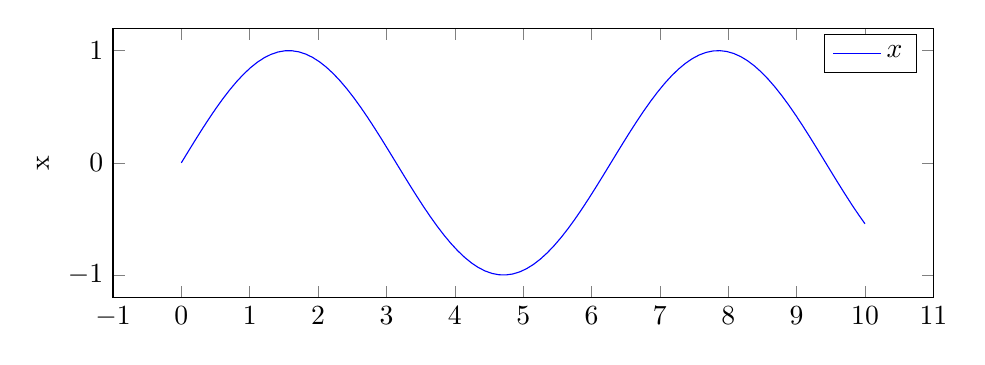
\begin{tikzpicture}
     \begin{axis}[width=12cm,height=5cm,ylabel=x] 
     \addplot[blue,domain=0:10,samples=100]{sin(deg(x))};
  \legend{$x$}
     \end{axis}
   \end{tikzpicture}
   \end{block}
   
\end{frame}

\begin{frame}
\frametitle{4D- Datenassimilation}
\vspace*{-0.1cm} 
    \begin{block}{Voraussetzung}
    \parbox[c][3.5\baselineskip][t]{\textwidth}{
     \begin{itemize}
     \item $\dot{x} = F(x),~ x_0 = x(0),~F\in C^1(\R^n)$
     \item $x_{obs}(t)$ - Observierungsparameter (Funktion oder diskrete Werte)
%      \item $C$ - Projektion von $X_{\text{State}}$ nach $X_{\text{Obs}}$ 
    \end{itemize}
    } 
   \end{block}
   \vspace*{-0.1cm} 
   \begin{block}{Problem}
      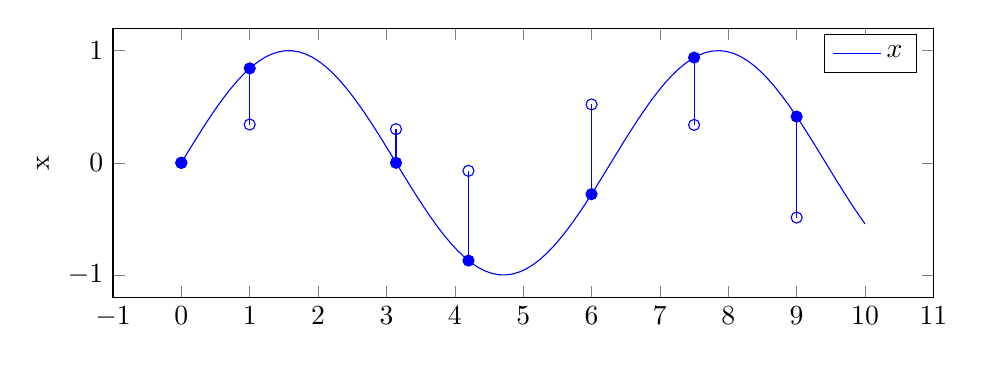
\begin{tikzpicture}
     \begin{axis}[width=12cm,height=5cm,ylabel=x] 
     \addplot[blue,domain=0:10,samples=100]{sin(deg(x))};
     \addplot+[blue,draw=none,mark=*, mark options={blue},error bars/.cd, y dir=plus,y explicit,error mark=o,error mark options={blue,mark size=2pt}] 
     coordinates { 
      (0,0) +- (0,0) 
     (1,0.8415) +- (0.5,-0.5) 
     (3.14,0) +- (0.05,0.3) 
     (4.2,-0.8715) +- (0,0.8)
     (6.0,-0.27942) +- (0,0.8)
     (7.5,0.93799) +- (0.1,-0.6) 
     (9,0.41212) +- (0.3,-0.9)}; 
  \legend{$x$}
     \end{axis}
   \end{tikzpicture}
   \end{block}
\end{frame}



\begin{frame}[<+->]
  \frametitle{Datenassimilation Schritte}
	\begin{block}{Ziel: Minimiere Kostenfunktional}
	\begin{equation}\label{eq:costFunctional}
		\min_{x_o} J(x_0) = \min_{x_o} \frac{1}{2}\int_0^T \|Cx(t) - x_{Obs}(t)\|^2dt
	\end{equation}
	  $C$ - Projektion von $X_{\text{State}}$ nach $X_{\text{Obs}}$ um eine sinnvolle Extrapolation zu erhalten.
	\end{block}
% 	\begin{block}{Datenassimilation Schritte}
% 	\begin{enumerate}
% 	 \item Berechnung Kostenfunktional
% 	 \item Berechnung $\nabla J(x_0)$
% 	 \item Optimierung
% 	\end{enumerate}
% 	\end{block}
\end{frame}
 
\begin{frame}[<+->]
  \frametitle{Datenassimilation Schritte}
  \begin{block}{Lösen einer ODE - z.B. Implizite Mittelpunktsregel(IMP)}
	\begin{equation}
	 x_n = x_a + h F \left(0.5 (x_a + x_n), t + 0.5 h\right)
	\end{equation}
	Speichere Werte $x_i$, berechne $J(x_0)$ mittels numerischer Quadratur
  \end{block}
  \begin{block}{Berechnung des Gradienten $\nabla J(x_0)$}
	Integriere das inhomogene adjungierte Tangent Linear Model rückwärts in $t$
	\begin{equation}
	  \dot{ \bar{x}}(t) =  -\frac{\partial F(x(t))}{\partial x}^\tr \bar x(t) +C^\tr(Cx(t) - x_{\text{obs}}(t)), ~ \bar x(T) =0
	\end{equation}
	\[
	\text{mit }\nabla J(x_0) = -\bar x(0)
	\]
  \end{block}
  \begin{block}{Optimierung}
  Finde $\argmin_{x_0} J(x_0)$ mit geeignetem Optimierungsverfahren (z.B. BFGS)
% 	Optimiere $x_0$ mit einem geeigneten Verfahren über $J$ mit $\nabla J$ (z.B. BFGS)
  \end{block}

\end{frame} 

\begin{frame}[<+->]
  \frametitle{Problemstellung}
  \begin{block}{Problemstellung}
  \centering
	Wie kann die Datenassimilation für den Fall
	\[
	  \dot{x} = F(x),~ x_0 = x(0),~F\in C^{0,1}(\R^n)
	\]
	betrachtet werden?
  \end{block}
%   \begin{block}
   \begin{itemize}
    \item Unglatte Modelle in Ingeneursdisziplinen z.B. Elektrotechnik (Diode)
    \item Ortsdiskretisierungen partieller Differentialgleichungen erster Ordnung ($\to$ Shallow Water Equation)
   \end{itemize}

%   \end{block}

\end{frame} 
